\documentclass{article}
\usepackage[utf8]{inputenc}
\usepackage[usenames]{color}
\usepackage{graphicx}
\usepackage{natbib}
\usepackage{amsmath}
\usepackage{amsfonts}
%\pagenumbering{gobble}%

% CSCI 8331 %

% avoid counting on sections %
\setcounter{secnumdepth}{-1}  
\title{Trying different functions for Pollard's rho integer factorization}
\author{Jos? Silveira \\
  George Washington University,\\
  \texttt{silveiraneto@gwu.edu}}
  
\date{\vspace{-5ex}}

\begin{document}

\maketitle

\begin{abstract}
This work measures empirically how the performance and accuracy changes with different functions for the Pollard's Rho integer factorization. It finds that $f(x) = x+\sqrt[]{n}$ is a better function than the original function proposed for this algorithm. This is the final work for the class CSCI 8331 Advanced Cryptography at George Washington University with professor Poorvi Vora. 
\end{abstract}

\section{Introduction}

Pollard's rho algorithm is a integer factorization algorithm that uses concepts from Floyd's cycle-finding algorithm and the Birthday Paradox. In algorithm receives an integer $n$ and returns a non trivial divisor of $n$ (i.e. not $1$) or $False$, which means it may have found a prime. Pollards rho of $n$ execution time varies because the probability of founding a divisor is not the same every number, as shown in $Figure\ 1$.

\begin{figure}[h!]
\centering
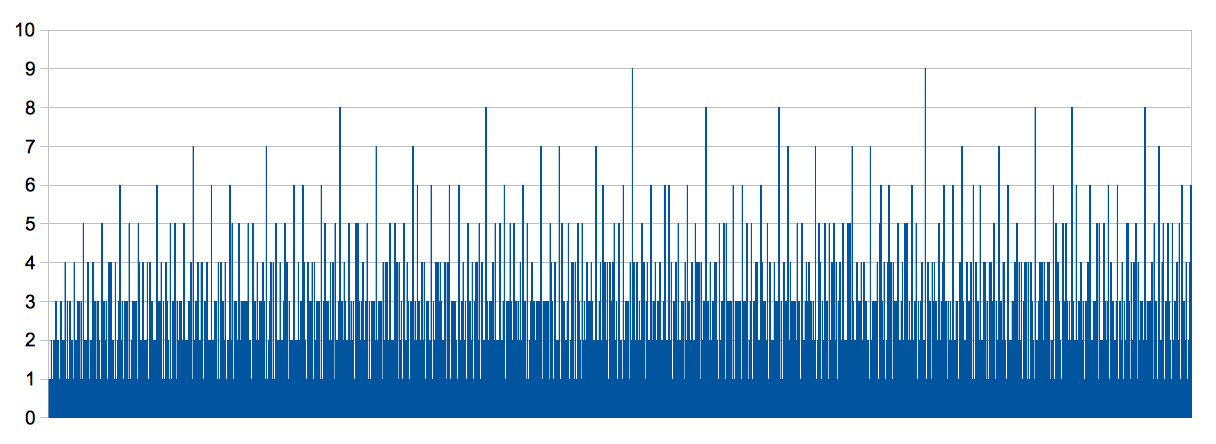
\includegraphics[scale=0.35]{factors.png}
\caption{Number of non trivial factors from 1 to 1000}
\label{fig1}
\end{figure}


\section{Functions}

All the functions $f_i$ are $modulo\ n$. The function tested were:\\
\begin{itemize}
  \item $f_1(x) = x^2-1$
  \item $f_2(x) = x^2+1$
  \item $f_3(x) = x^3-1$
  \item $f_4(x) \xleftarrow{R} \mathbb{N}$
  \item $f_5(x) = 4x^2 - 2x +41$
  \item $f_6(x) = x+1$
  \item $f_7(x) = x+2$
  \item $f_8(x) = x+\sqrt[]{n}$
  \item $f_9(x) = 2**x$
  \item $f_{10}(x) = 2**x+1$
  \item $f_{11}(x) = 2x$
  \item $f_{12}(x) = 3x$
  \item $f_{13}(x) = x+3$
  \item $f_{14}(x) = 4x$
  \item $f_{15}(x) = x**2+3$
\end{itemize}

$f_1$ is the original function presented by Pollard \citep{pollard1975monte}. $f_2$ is a common variation. $f_4(x)$ test the hypothesis that $f_1$ was originally chosen because it behaves like a random function. $f_5$ uses the Euler's prime equation. $f_6$ is the consecutive function that guarantees that all numbers will be examined. $f_{15}$ is the function empirically chosen by Brent \citep{brent1980improved}.

\section{Methodology}

For each function, two parameters were analysed, the fail rate and the performance. The fail rate is how many times the pollard's rho fails, i.e. returns an incorrect divisor or returns \textit{False} when the input is not a prime. In the experiments, the pollard's rho method never returned a wrong divisor but depending on the chosen function it can return a false prime. In a practical implementation of this method a fail rate would not be acceptable, requiring to run the method more times using other functions until it returns a divisor or giving it up and assuming the input was a prime. This would imply a bad worst case scenario with prime numbers. In our implementation we accept the output of the method, but count the number of times it fails against a reliable prime verification. For this results, a fail rate higher than zero means that the performance in a practical implementation would be even worst.\\

The second parameter analysed was the performance for $100$ execution trials. The benchmark was done using the \textit{timeit} benchmark library for Python which avoids a number of common traps for measuring execution times. Each trial for a function was composed of the execution of pollard's rho method using the function for values between $2$ and $1000$.\\

Measurements were made using a Amazon Web Services EC2 instance of compute optimized type c3.2xlarge with High Frequency Intel Xeon E5-2670 v2 (Ivy Bridge) Processors, 8 vCPU, and 15Gb RAM. Due the serial nature of this algorithm and its insignificant memory requirements this setup was highly above the minimum necessary but it could run the benchmark 100 times faster than the development desktop.\\

\section{Implementation}

The \textit{Python} implementation used for this benchmark and raw results can be found at https://github.com/silveira/pollardsrho.

\section{Results}

The results for each function and their respective fail rate and performance:\\

\begin{tabular}{l*{2}{c}r}
Function              & Fail rate & Performance \\
\hline
$f_1(x)$ & 3.0\% & 0.756325960159 \\ 
$f_2(x)$ & 2.2\% & 0.771731138229 \\ 
$f_3(x)$ & 3.1\% & 3.81694221497 \\ 
$f_4(x)$ & 0.6\% & 44.762458086 \\ 
$f_5(x)$ & 1.9\% & 0.774783849716\\ 
$f_6(x)$ & 0\% & 11.6375050545 \\ 
$f_7(x)$ & 0\% & 11.491779089 \\ 
$f_8(x)$ & 0\% & 0.443336009979 \\ 
$f_9(x)$ & 5.5\% & 11.4220769405 \\ 
$f_{10}(x)$ & 4.4\% & 8.37259697914 \\ 
$f_{11}(x)$ & 0\% & 7.15102696419 \\ 
$f_{12}(x)$ & 0\% & 7.26384687424 \\ 
$f_{13}(x)$ & 0\% & 11.4748301506 \\ 
$f_{14}(x)$ & 0.4\% & 4.31600689888 \\ 
$f_{15}(x)$  & 2.1\% & 0.710178852081 \\ 
\end{tabular}

\section{Conclusion}

$f_8(x) = x+\sqrt[]{n}$ had the best result with lowest time execution and without any fails, which means that in a real application it would not be necessary to run the algorithm multiple times with different functions. With a simple optimization to memoize the value of $\sqrt[]{n}$ it would perform even better.

\begin{figure}[h!]
\centering
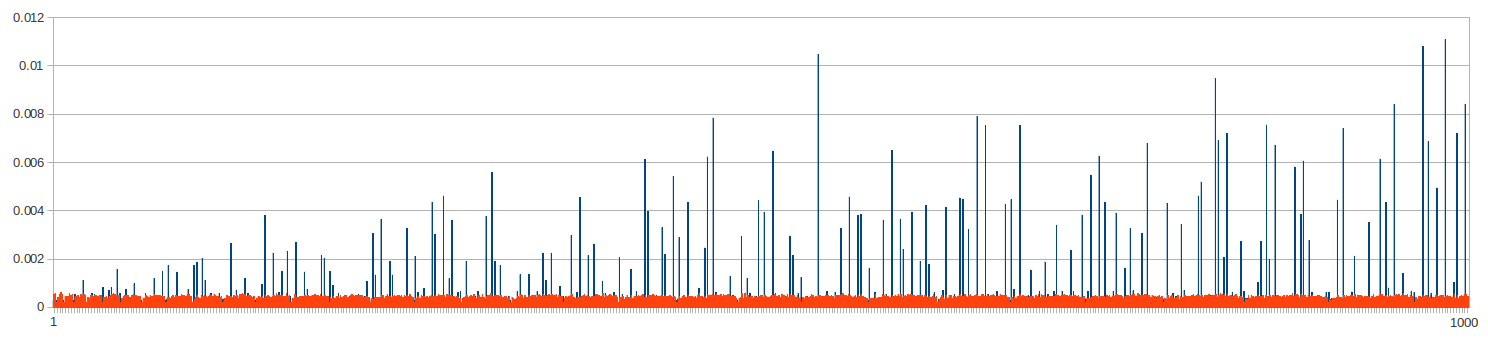
\includegraphics[scale=0.30]{f1_f8.png}
\caption{Execution times with inputs from 1 to 1000 for $f_1(x)$ (blue) and $f_8(x)$ (orange).}
\label{fig2}
\end{figure}

%------------------------------------------------------------------------------------------------------------------%


\bibliographystyle{plain}
\bibliography{references}

\end{document}

